\documentclass{beamer}
\usetheme{afm}

\title{Arbitrage-Free Pricing Theory}
\subtitle{Basic Definitions and a Bit of Stochastic Calculus}
\course{Advanced Financial Modeling}
\author{\href{mailto:matteo.sani@unisi.it}{Matteo Sani}}

\begin{document}
	\begin{frame}[plain]
		\maketitle
	\end{frame}

%\AtBeginSection{
%\begin{frame}{Outline}
%	\begin{multicols}{2}
%		\tableofcontents
%	\end{multicols}
%	\tableofcontents%[currentsection]
%\end{frame}
%}

\section{Random Variables}
\begin{frame}{Random Variables}
	\begin{block}{Definition}
	A variable whose value is a number determined by the outcome of a random experiment is called a \textcolor{red}{random variable}.
	\end{block}
	\vspace{0.5 cm}
        
	\pause
	Random variables are very different from usual \emph{algebraic variables}:
\begin{equation*}
	x^2 - 3 = 0 \implies x = \pm \sqrt{3}
\end{equation*}	
	no matter how many times I solve this equation.
\end{frame}

\begin{frame}{Random Variables}
	A random variable instead is kind of a mapping between 
	\begin{equation*}
		X(\omega):\Omega\rightarrow \mathbb{R}\quad \forall\omega\in\Omega
	\end{equation*}
	such that $X(\omega)$ represents the occurrence probability of the "outcome" $\omega$. $\Omega$ is called \textcolor{red}{sample space} and is the set of all possible future states (or outcomes) of a process.
	\pause
	\vspace{0.5cm}
        
	Hence the random variable $X$ will take values distributed according to the probability distribution of the random process, e.g. if $X$ represents the outcomes of rolling a \emph{fair} die $\Omega = [1,2,3,4,5,6]$ and each value has equal probability of 1/6.
	\vspace{0.5cm}
        
	\textcolor{red}{A random variable is always associated to a probability distribution.}
%	There are two kinds of random variable:
%	\begin{itemize}
	%		\item Discrete Random Variable
	%		\item Continuous Random Variable
	%	\end{itemize}
\end{frame}

\subsection{Properties and Characteristics of Random Variables}
\begin{frame}{Discrete and Continuous Random Variables}
	\begin{block}{Definition} 
		If a random variable takes only a countable number (finite) of values, it is called \textcolor{red}{discrete}.
	\end{block}
	
	\small{
		\textbf{Example:} when 3 coins are tossed, the number of heads obtained is the random variable, which assumes the values $\Omega=\{0,1,2,3\}$ ($\Omega$ ia a countable set).}
	\newline
	\pause
	\begin{block}{Definition} 
		A random variable $X$ which can take any value between a certain interval is called \textcolor{red}{continuous}.
	\end{block}
	
	\small{\textbf{Example:} the height of students in a particular class lies between 160 and 190~cm $(X = \{x|160 \leq x \leq 190\})$.}
\end{frame}

\begin{frame}{Probability Distribution}
	Let $X$ be a random variable defined on a domain $\Omega$ of possible outcomes. 
	\renewcommand{\arraystretch}{1.6}
	\begin{table}[bt]
		\begin{tabular}{|c|c|} \hline
			\textbf{Discrete} & \textbf{Continuous} \\ \hline
			Probability Mass & Probability Density \\ \hline		
			$P(X=x_i)\;\forall x_i\in\Omega$ & $P(X=x)=\int_x^{x+dx}f(x)dx$ \\ \hline
			$P(x_i) \geq 0;\;\forall i$ & $f(x) \geq 0;\;-\infty < x < \infty$\\ \hline
			$\sum_{i=0}^{n} P_i = 1$ & $\int_{-\infty}^{\infty} f(x) dx = 1$\\ \hline
			\multicolumn{2}{|c|}{Cumulative Distribution} \\ \hline
			$F(x_i) = P(X<x_i) = \sum_{x<x_i} P(x)$ & $F(x) = P(X<a) = \int_{-\infty}^{a} f(x) dx$ \\ \hline
		\end{tabular}
	\end{table}
	\begin{tikzpicture}[remember picture,overlay]
	\node[xshift=5cm,yshift=-3.7cm] (image) at (current page.center) {
\includegraphics[width=20px]{python_logo}};
	\node[align = center, yshift=1.45cm, below=of image] {\tiny{\href{shorturl.at/JR059}{shorturl.at/JR059}}};
\end{tikzpicture}
\end{frame}

\begin{frame}{Characterizing a Random Variable}
	If we know the distribution of a random variable, we pretty much know all is needed about it. 
	\newline
	\begin{columns}
		\column{0.45\linewidth}
		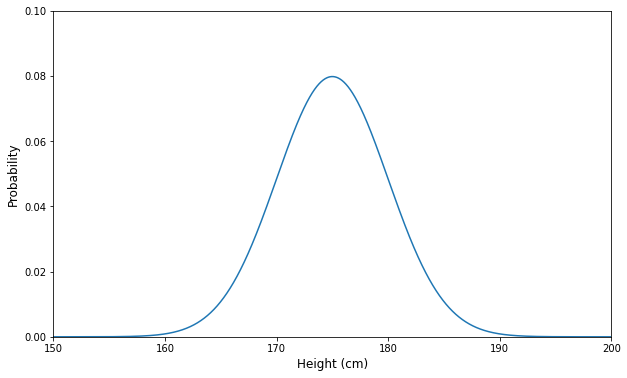
\includegraphics[height=3cm]{continouos_random_variable}
		\pause
		\column{0.45\linewidth} 
		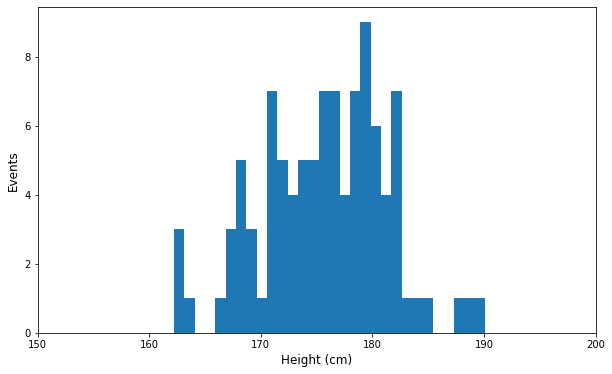
\includegraphics[height=3 cm]{real_data}
	\end{columns}
	\vspace{0.5cm}
        
	But with \textit{real data}, we don't know the full distribution. Fortunately we can characterize it by a couple of numbers (\emph{statistics}).
	\pause
	\small{
		\begin{center}
			\textcolor{red}{mean:} $\boxed{\mu = \mathbb{E}[X] = \int_{-\infty}^{\infty} xf(x)dx}$\quad
			\textcolor{red}{variance:}  
			$\boxed{\sigma^2 = \mathbb{E}[(X-\mu)^2] =\int_{-\infty}^{\infty} (x-\mu)^2f(x)dx}$
	\end{center}
}
\end{frame}

\subsection{Expectation and Its Properties}
\begin{frame}{Properties of Expectation}
	\renewcommand{\arraystretch}{1.4}
	{\tiny {\tiny }}{
		\begin{table}[bt]
			\begin{tabular}{|c|c|} \hline
				Scalar multiplication & $\mathbb{E}[aX] = a\mathbb{E}[X]$ \\ \hline
				Sums & $\mathbb{E}[X_1+\ldots +X_K] =  \mathbb{E}[X_1] +\ldots + \mathbb{E}[X_n]$ \\ \hline
				Linear combinations & $\mathbb{E}[a_1X_1+\ldots +a_KX_K] =  a_1\mathbb{E}[X_1] +\ldots + a_K\mathbb{E}[X_K]$ \\ \hline
				Expected value of a constant & $\mathbb{E}[a] = a$ \\ \hline
				Products (independent variables) & $\mathbb{E}[XY] = \mathbb{E}[X] \mathbb{E}[Y]$ \\ \hline
			\end{tabular}
		\end{table}
	}
	Essentially all the expectation properties come from integration properties, e.g.
	\begin{equation*}
		\mathbb{E}[aX] = \int_{-\infty}^{\infty} ax f(x) dx = a  \int_{-\infty}^{\infty} x f(x) dx = a\mathbb{E}[X]
	\end{equation*}
\end{frame}

\section{Stochastic Processes}
\begin{frame}{Stochastic Process}
	Real world data is noisy (i.e. distorted), and exhibits behaviours that cannot be described by a deterministic model (always produce same result from same inputs, e.g $f(x)=x^3+2$).
	\pause
	\begin{tabular}{cl}  
		\begin{tabular}{c}
			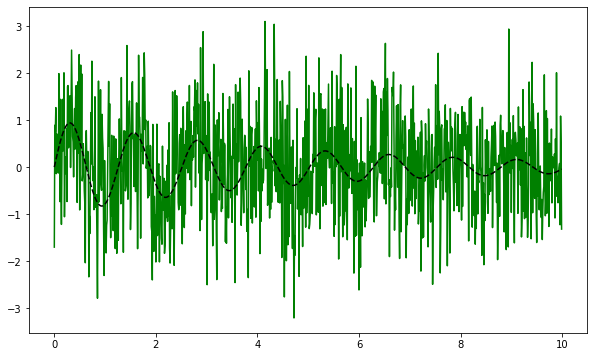
\includegraphics[height=3cm]{stochastic_process}
		\end{tabular}
		& \begin{tabular}{l}
			\parbox{0.45\linewidth}{
				Need to switch to \textcolor{red}{stochastic processes} in order to model the uncertainty of data.  
			}
		\end{tabular}  \\
	\end{tabular}
    \pause
	\begin{block}{Definition}
		A collection of random variables that is indexed by some mathematical set (usually time) is called a \textcolor{red}{stochastic processes}.
	\end{block}
\end{frame}

\subsection{SDE}
\begin{frame}{Stochastic Differential Equation}
	
	Stochastic processes are described by \emph{stochastic differential equations} (SDE):
	
	\begin{equation*}
		\begin{aligned}
			dX(t) = \mu(t,X(t)) dt &+ \sigma(t,X(t)) dW(t) =\\  & =\underbrace{\mu(t,X(t))dt}_{\textrm{deterministic}} + \underbrace{\sigma(t,X(t)) \mathcal{N}(0,1)\sqrt{dt}}_{\textrm{stochastic}}
		\end{aligned}
	\end{equation*}
	
	\begin{tabular}{cl}  
		\begin{tabular}{c}
			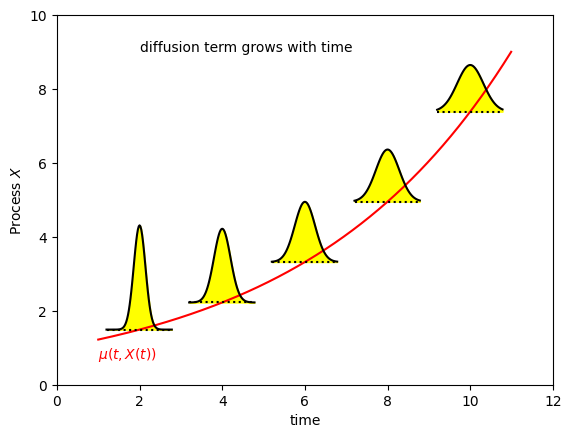
\includegraphics[height=3.5cm]{brownian_process}
		\end{tabular}
		& \begin{tabular}{l}
			\parbox{0.45\linewidth}{
				\begin{itemize}
					\item The mean of $dW$ is zero and its variance is $dt$
					\item the standard deviation grows with the square root of time: $W(t) \simeq \mathcal{N}(0, t)$ because each $dW$ is distributed like independent standard Gaussian.
				\end{itemize}  
			}
		\end{tabular}  \\
	\end{tabular}
\end{frame}

\subsection{Martingales}
\begin{frame}{Martingale}
	\begin{block}{Definition}
		A \textcolor{red}{martingale} is a (integrable and adapted) stochastic process which models a fair game with the following remarkable feature
		\begin{equation}
			\mathbb{E}[X_t|\mathcal{F}_s] = X_s
		\end{equation}
		so the best prediction for the future value $X_t$, given the knowledge $\mathcal{F}_s$ at time $s$ is the value at time $s$ itself, $X_s$.
	\end{block}
\end{frame}

\begin{frame}{Martingale}
	\begin{block}{Properties}
		If $X_t$ is a stochastic process with diffusion coefficient (i.e. volatility) $\sigma_t$, which satisfies $\mathbb{E}\left[\left(\int_0^T\sigma^2_s ds\right)^{\frac{1}{2}}\right]<\infty$, and SDE $dX_t=\mu_t dt+\sigma_t dW_t$ 
		\begin{equation*}
			X\text{ is a martingale } \iff X\text{ is drift-less } (\mu_t=0)
		\end{equation*}
	\end{block}	
	A martingale corresponds to the common notion that "an efficient price, changes randomly" so we cannot know if it will go up or down. That is why this mathematical concept is brought into finance.
	
	\begin{tikzpicture}[remember picture,overlay]
		\node[xshift=-5cm,yshift=-3.7cm] (image) at (current page.center) {
\includegraphics[width=20px]{python_logo}};
		\node[align = center, yshift=1.45cm, below=of image] {\tiny{\href{shorturl.at/knyGT}{shorturl.at/knyGT}}};
	\end{tikzpicture}
\end{frame}

\subsection{Geometric Brownian Motion (GBM)}
\begin{frame}{Geometric Brownian Motion}
	\begin{itemize}
		\item<0-> Trade random fluctuations deviate a stock price $S_t$ from a steady state.
		\item<0-> The price relative change in $dt$ can be decomposed into two parts
		\begin{itemize}
			\item<2-> \textcolor{red}{deterministic}: the expected return from holding the stock during $dt$. It can be expressed as $\mu S_tdt$ (with $\mu$ being the expected rate of return);
			\item<3-> \textcolor{red}{stochastic}: models the random changes of the market. A reasonable assumption is to equal this term to $\sigma S_t dW_t$. 
		\end{itemize}
		\item<4-> Putting all together, the resulting SDE is
		\begin{equation}
			\begin{gathered}
				dS_t = \mu S_t dt + \sigma S_t dW_t \\
				\frac{dS_t}{S_t} = d\log(S_t) = \mu dt + \sigma dW_t
			\end{gathered}
			\label{eq:log_normal_sde}
		\end{equation}
	\end{itemize}
\end{frame}

\subsubsection{It$\hat{o}$'s Formula}
\begin{frame}{It$\hat{o}$'s Formula}
	\begin{block}{Proposition}
		For any given continuous and differentiable function $G(S,t)$ where S satisfies $dS=adt + bdW_t$, holds
		\begin{equation}
			dG = \left(a\frac{\partial G}{\partial S} + \frac{\partial G}{\partial t} + \underbrace{\frac{1}{2}b^2\frac{\partial^2 G}{\partial S^2}}_{\text{additional term}}\right)dt + b\frac{\partial G}{\partial S} dW
			\label{Eq:itos_lemma}
		\end{equation}
	\end{block}
	
	This is essentially an extension of the \emph{Taylor series} for stochastic functions, in the expansion an extra term appears.
\end{frame}

\begin{frame}{It$\hat{o}$'s Formula "Proof"}
	\begin{itemize}
	\item Suppose $X_t$ is an stochastic process that satisfies the SDE
	\begin{equation*}	
	dX_{t}=\mu _{t}\,dt+\sigma _{t}\,dW_{t}
	\end{equation*}.
	\item If $f(t,x)$ is a twice-differentiable scalar function of $X$, its expansion in a Taylor series is
	\begin{equation*}
	df={\frac {\partial f}{\partial t}}\,dt+{\frac {1}{2}}{\frac {\partial ^{2}f}{\partial t^{2}}}\,dt^{2}+\cdots +{\frac {\partial f}{\partial x}}\,dx+{\frac {1}{2}}{\frac {\partial ^{2}f}{\partial x^{2}}}\,dx^{2}+\cdots
	\end{equation*}
	\item Substituting $X_t$ for $x$ and $dX_t$ with the SDE gives
	\begin{equation*}
		\begin{aligned}
		df&={\frac {\partial f}{\partial t}}\,dt+{\frac {1}{2}}{\frac {\partial ^{2}f}{\partial t^{2}}}\,dt^{2}+\cdots +{\frac {\partial f}{\partial x}}(\mu _{t}\,dt+\sigma _{t}\,dW_{t})+\\
		&+{\frac {1}{2}}{\frac {\partial ^{2}f}{\partial x^{2}}}\left(\mu _{t}^{2}\,dt^{2}+2\mu _{t}\sigma _{t}\,dt\,dW_{t}+\sigma _{t}^{2}\,dW_{t}^{2}\right)+\cdots
		\end{aligned}
	\end{equation*}
\end{itemize}
\end{frame}

\begin{frame}{It$\hat{o}$'s Formula "Proof"}
	\begin{itemize}
	\item Stopping the expansion up to the first order (i.e. negletting $dt^2$ and $dt dW_t$ terms), and collecting $dt$ and $dW$ terms, we obtain
	\begin{equation*}
	df=\left({\frac {\partial f}{\partial t}}+\mu _{t}{\frac {\partial f}{\partial x}}+{\frac {\sigma _{t}^{2}}{2}}{\frac {\partial ^{2}f}{\partial x^{2}}}\right)dt+\sigma _{t}{\frac {\partial f}{\partial x}}\,dW_{t}
	\end{equation*}
	as required.
\end{itemize}
\end{frame}

\begin{frame}{Geometric Brownian Motion}
	\begin{itemize}
		\item<0-> Let's apply this expansion to $G=\log(S_t)$ 
		\begin{equation*}
			\frac{\partial G}{\partial S}=\frac{1}{S_t},\;\frac{\partial G}{\partial t}=0,\;\frac{\partial^2 G}{\partial S^2}=-\frac{1}{S_t^2}
		\end{equation*}
		\item<2-> Substituting back into It$\hat{o}$'s lemma \cref{Eq:itos_lemma} and taking $a$ and $b$ values from \cref{eq:log_normal_sde}
		\begin{equation*}
			dG = \left(a\frac{\partial G}{\partial S} + \frac{\partial G}{\partial t} + \frac{1}{2}b^2\frac{\partial^2 G}{\partial S^2}\right)dt + b\frac{\partial G}{\partial S} dW
		\end{equation*}
	\end{itemize}
	\pause
	\pause
	\begin{equation*}
	d(\log S_t) = \left[\mu S_t\frac{1}{S_t} + \frac{1}{2}\sigma^2S_t^2\left(-\frac{1}{S_t^2}\right)\right]dt + \sigma dW
	\end{equation*}
	\pause
	\begin{equation*}
	\log(S_t) - \log(S_{t-1}) = \log\frac{S_t}{S_{t-1}}=\left(\mu - \frac{1}{2}\sigma^2\right)dt + \sigma dW 
	\end{equation*}	
	\pause
	\begin{equation}
	S_t = S_{t-1}\exp\left[\left(\mu-\frac{1}{2}\sigma^2\right)dt + \sigma\mathcal{N}(0,1)\sqrt{dt}\right] 
	\label{eq:lognormal_solution}
	\end{equation}
\end{frame}

\subsubsection{Log-normality}
\begin{frame}{Log-normality}
	\begin{itemize}
		\item The variation in $\log(S_t)$ equals a constant (the \emph{drift} $\mu-\frac{1}{2}\sigma^2$) plus a Gaussian distributed random variable. Therefore at some time $t$
		\begin{equation*}
			\log S_t = \mathcal{N}\left[\left(\mu -\frac{\sigma^2}{2}\right)t, \sigma^2 t\right]
		\end{equation*}
	\end{itemize}
	\pause
	\begin{block}{Definition}
		A random variable whose logarithm is normally distributed is said to be \textcolor{red}{log-normal}.
		
		One of the most important properties of a log-normal distribution is to be positive definite (a good characteristic for stock prices).
	\end{block}
	\begin{tikzpicture}[remember picture,overlay]
		\node[xshift=5cm,yshift=-3.7cm] (image) at (current page.center) {
\includegraphics[width=20px]{python_logo}};
		\node[align = center, yshift=1.45cm, below=of image] {\tiny{\href{shorturl.at/htCFJ}{shorturl.at/htCFJ}}};
	\end{tikzpicture}
\end{frame}

\begin{frame}{Final Remark on Stochastic Processes}
\begin{center}
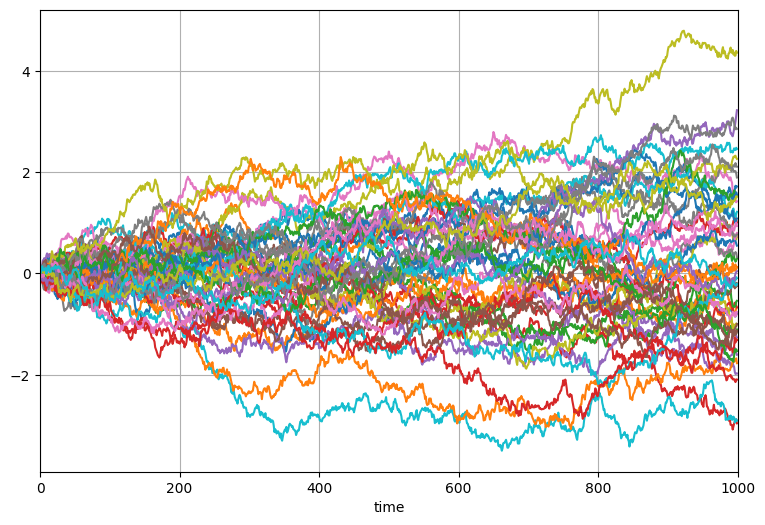
\includegraphics[width=0.45\linewidth]{sde_simulations}
\end{center}
When you have to get something out of a stochastic process you cannot rely on a single realization. 
Instead you need to take into account "all" the possible paths the process can go through in a \emph{statistical} way with an \textcolor{red}{expectation ($\mathbb{E}$)}. 
Hence it is mandatory to know (or assume) the \textcolor{red}{proper probability distribution}.
\end{frame}
	

\section{No Arbitrage Theory}
\subsection{No Arbitrage Principle\ldots}

\begin{frame}{Disclaimer}
  When it comes to making things sound and look much more complicated than they are, financial maths really does reign supreme. Fortunately it’s not just me who thinks it’s all overly complicated but even Paul Wilmott \href{https://wilmott.com/science-in-finance-viii-the-maths-sweet-spot/}{thinks the profession takes it just a bit too far} and he’s a bit better at maths than me.\vspace{0.5cm}
  
\pause
As an example, this is number one recommended \textcolor{red}{easier} way to to remember what the risk-neutral measure is on Wikipedia:

\pause{\emph{"The probability measure of a transformed random variable. Typically this transformation is the utility function of the payoff.}}
\pause{\emph{The risk-neutral measure would be the measure corresponding to an expectation of the payoff with a linear utility."}}
\end{frame}

\begin{frame}{Portfolio}
	\begin{block}{Definition}
		A \textcolor{red}{portfolio} is a vector $\mathbf{\theta}\in \mathbb{R}^K$ whose $j$ components represent the number of shares of asset $A_j$ (asset $A_0$ is risk-free). It's value is
		\begin{equation}
			V_t(\mathbf{\theta}, \omega)=\sum_{j=1}^K\theta_jS^j_t(\omega)
		\end{equation} 
		where $S_t^j$ is the value of $j$-th asset, and $\omega$ a market situation. A portfolio is \textcolor{red}{self-financing} if its value changes only due to variations of the asset prices.
	\end{block}
\end{frame}

\begin{frame}{Arbitrage}
	\begin{block}{Definition}
		An \textcolor{red}{arbitrage} is a self financing portfolio $\mathbf{\theta}$ such that
		\begin{equation}
		%V_0(\mathbf{\theta}, \omega)\le 0 \text{ and } \mathcal{P}\{V_t(\mathbf{\theta}, \omega) > 0\} > 0
		P(V_{t}\geq 0)=1{\text{ and }}P(V_{t}\neq 0)>0,\,0<t\leq T
		\end{equation}
		where $V_0=0$, $V_t$ denotes the portfolio value at time $t$ and $T$ is the time the portfolio ceases to be available on the market. This means that the value of the portfolio is never negative, and guaranteed to be positive at least once over its lifetime.
	\end{block}
    \pause
	Informally, \textcolor{red}{arbitrage is a way to make a guaranteed profit from nothing}, by short-selling certain assets at time $t = 0$, using the proceeds to buy other assets, and then settling accounts at time $t$. 
	\small{Arbitrage may take place when: the same asset does not trade at the same price on all markets, or two assets with identical cash flows do not trade at the same price}.
\end{frame}

\subsection{Fundamental Theorems of Arbitrage Pricing}
\begin{frame}{Fundamental Theorems of Arbitrage Pricing}
	\begin{block}{Theorem I}
		There exists a \emph{risk-neutral measure} if and only \textcolor{red}{if arbitrages do not exist}.
	\end{block}
	\pause
	\vspace{1cm}
        
    We are assuming the market doesn't allow for risk-free profits with no initial investment.
    Indeed arbitrage opportunities rarely exist in practice. If and when they do, gains are extremely small (not for small investors), and are typically short-lived and difficult to spot. 

    \pause
    \textcolor{red}{Arbitrage exclusion in the mathematical model is close enough to reality}.
	
    \pause
    But what does it mean "risk-neutral measure" ?
\end{frame}

%\begin{frame}{Few Definitions}
%	TOGLIERE
%	\begin{block}{Definition}
%		A \textcolor{red}{numeraire} is any positive non-dividend-paying asset. It is a reference asset chosen to normalize all other asset prices to it. Having a numeraire allows for the comparison of the value of goods against one another.
%	\end{block}
%    METTERE NELLE SLIDE DOPO
%    \begin{block}{Definition}
%		A \textcolor{red}{probability measure} is a real-valued function that assignes probabilities to a set of events in a sample space that satisfies measure properties such as countable additivity, and assigning value 1 to the entire space.
%	\end{block}	
%\end{frame}

\begin{frame}{Risk Neutral Measure}
	\begin{itemize}
	\item<1-> Prices of assets depend crucially on their risk as investors typically demand more profit for bearing more risk.
        \item<2-> Therefore, today's price of a claim on a risky amount realized tomorrow will generally differ from its expected value.
        \item<2-> Most commonly, investors are risk-averse and today's price is below the expectation, remunerating those who bear the risk.
	\item<4-> Consequently to price assets, the calculated expected values need to be adjusted for an investor's risk preferences
        \item<5-> Unfortunately, these adjustments would vary between investors and an individual's risk preference is very difficult to quantify.
	\item<6-> \textcolor{red}{It turns out that, under few assumptions, there is an alternative way to do this calculation.}
	\end{itemize}
\end{frame}

\begin{frame}{Risk-Neutral Measure}
Denote the risk-free rate with $r$ and assume today's stock price to be $S_0$. In one period of time from now, the price could be 
\begin{equation*}
	\begin{cases}
		S_0\cdot u = S_u \\
		S_0\cdot d = S_d \\ 
	\end{cases}, \quad \text{with }(u > d)
\end{equation*}
\pause
To \emph{avoid arbitrage opportunities}, conditions must be imposed on $u$ and $d$. 

(Example: in case $e^r > u$, I could short the stock in $t_0$ and invest the proceeds $S_0$ into the risk-free account: in both future states in $t_1$, I could buy the stock back for less than my proceeds $S_0e^r$ because $S_u$ and $S_d$ would both be lower. Similarly for $e^r < d$\ldots)
\pause

So \textcolor{red}{imposing $d\le e^r \le u$, will ensure no arbitrage}.
\end{frame}


\begin{frame}{Risk-Neutral Measure}
\begin{equation*}
	\begin{aligned}
	S_0 &= \frac{S_0(u-d)e^r}{(u-d)e^r} = \frac{S_0(u-d)e^r + (S_0ud - S_0ud)}{(u-d)e^r}=\\
	&= \frac{1}{e^r}\left(\frac{S_0ue^r - S_0ud}{u-d} + \frac{-S_0de^r + S_0ud}{u-d}\right)=\\
	&= \frac{1}{e^r}\left(S_0u\frac{e^r - d}{u-d} + S_0d\frac{u - e^r}{u-d}\right)
	\end{aligned}
\end{equation*}
\pause
The no arbitrage condition implies the following bounds
\begin{equation*}
0\le\frac{e^r -d}{u-d}\le 1,\quad 0\le\frac{u - e^r}{u-d}\le 1
\end{equation*}
\pause
also
\begin{equation*}
 \frac{e^r -d}{u-d} + \frac{u - e^r}{u-d} = 1
\end{equation*}
\end{frame}

\begin{frame}{Risk-Neutral Measure}
  So we can interpret $p_u=\cfrac{e^r -d}{u-d}$ and $p_d=\cfrac{u - e^r}{u-d}$ as \textcolor{red}{(risk-neutral) probability measure} ($\mathcal{Q}$).\vspace{0.3cm}
  
\pause
\begin{block}{Definition}
	A \textcolor{red}{probability measure} is a real-valued function that assigns probabilities to a set of events in a sample space that satisfies measure properties such as countable additivity, and assigning value 1 to the entire space.
\end{block}	
\pause
Rewriting previous expression of $S_0$ in terms of the newly defined probabilities
\begin{equation}
S_0 = \frac{S_up_u + S_dp_d}{e^r} = e^{-r}\mathbb{E}^\mathcal{Q}[S_1]
\label{eq:risk_neutral_price}
\end{equation}

So the stock price, "under the chosen probability measure" is the discounted stock expectation at $t_1$.
\end{frame}

\begin{frame}{Risk-Neutral Measure}
%We have never talked about the probabilities of the stock going up or down; every investor might have her view of the world with different probabilities assigned to the stock. 

The \textcolor{red}{risk-neutral measure} is agreed upon by the market as a whole just as a consequence of no arbitrage assumption.
In other words it is nothing more than an \emph{implied probability distribution}.
\pause

Implied from observable prices of tradable instruments, and used to determine \textcolor{red}{objective fair prices} for an asset or financial instrument. Probabilities are assessed with the risk taken out of the equation, so it doesn’t play a factor in the anticipated outcome.
\pause

By contrast, if you tried to estimate the anticipated value of a stock based on how likely it is to go up or down, considering unique factors or market conditions that influence that specific asset, you would be including risk into the equation and, thus, would be looking at \textcolor{red}{real or physical probability}.
\end{frame}

\begin{frame}{Risk-Neutral Measure and Pricing}

\begin{block}{Proposition}
	Assume there exists a \textcolor{red}{risk-neutral measure} $\mathcal{Q}^0$ %on the set $\Omega$ of possible market scenarios 
	and let $A$ be an asset. Then, for each time $t$, $0\le t\le T$ there exists a unique price $\pi_t$ associated with $A$
	\begin{equation}
		\pi_t = \mathbb{E}^{\mathcal{Q}^0}[D(t,T)V_A|\mathcal{F}_t]
		\label{eq:risk_neutral_pricing}
	\end{equation}
\end{block}

Such a price is given by the expectation of the discounted payoff under the measure $\mathcal{Q}^0$.

Note that $\mathcal{F}_t$ is called \textcolor{red}{filtration} and represents our knowledge of the system up to time $t$, i.e. the expectation is indeed \emph{conditioned} to what happened until time $t$.
%The benefit of this risk-neutral pricing approach is that once the risk-neutral probabilities are calculated, they can be used to price every asset based on its expected payoff. These theoretical risk-neutral probabilities differ from actual real-world probabilities, which are sometimes also referred to as physical probabilities. If real-world probabilities were used, the expected values of each security would need to be adjusted for its individual risk profile.

%You might think of this approach as a structured method of guessing what the fair and proper price for a financial asset should be by tracking price trends for other similar assets and then estimating the average to arrive at your best guess. 

%For this approach, you would try to level out the extreme fluctuations at either end of the spectrum, creating a balance that creates a stable, level price point. You would essentially be minimizing the possible unusual high market outcomes while increasing the possible lows.
\end{frame}

\begin{frame}{Risk-Neutral Measure and Pricing}
	\begin{itemize}
		\item Later in this course, in the context of the change of measure, we are going to formalize the previous slide statement.
		\item In summary, we will show a generalization of the original ideas of Black and Scholes, showing that, under complete markets with no arbitrage, it is possible to use for pricing purposes (only) stochastic models that do not factor in the risk premium.
		\item \textbf{Example:} imagine an asset such that $S_0=100$ and that $S_u=120$ and $S_d=80$. If the risk-free rate is 5\% the risk-neutral probability is 
		\begin{equation*}
		q = \frac{e^r - d}{u-d} \approx 63\%
		\end{equation*}
	\end{itemize}
%	\begin{tikzpicture}[remember picture,overlay]
%	\node[xshift=5cm,yshift=-3.7cm] (image) at (current page.center) {
\includegraphics[width=20px]{python_logo}};
%	\node[align = center, yshift=1.45cm, below=of image] {\tiny{\href{shorturl.at/htCFJ}{shorturl.at/htCFJ}}};
%	\end{tikzpicture}
\end{frame}

\begin{frame}{Hedging}
	\begin{itemize}
		\item A portfolio $\mathbf{\theta}$ in the assets $A$ is a \textcolor{red}{replicating portfolio} for the asset $B$ if
		\begin{equation}
			S_t^{B}(\omega_i) = \sum_{j=1}^K \theta_j S_t^j(\omega_i)\quad\forall i=1,2,\ldots,N
		\end{equation}
		\item In particular it can be demonstrated if the market is \emph{arbitrage-free} then the relation holds for all $t$.
		\item The importance of replicating portfolios is that they enable financial institutions that sell
		asset $B$ (e.g. a call options) to \textcolor{red}{hedge}: for each sold share of asset $B$, buy $\theta_j$ shares
		of asset $A_j$ and hold them to time $t + 1$. Then at time $t + 1$, 
		\begin{equation*}
			\text{net gain }= \text{ net loss } = 0
		\end{equation*}
	\end{itemize}
\end{frame}

\begin{frame}{Fundamental Theorems of Arbitrage Pricing}
	\begin{itemize}
		\item In some circumstances, an arbitrage-free market may admit more than one risk-neutral measure, i.e. \textcolor{red}{incomplete markets}.
		\item By contrast, a \textcolor{red}{complete market} is one that has a unique risk-neutral measure.
	\end{itemize}
	\pause
	\begin{block}{Theorem II}
		Let $\mathcal{M}$ be an arbitrage-free market with a risk-less asset. If for every derivative security there is a replicating portfolio in the assets $A_j$ then the market $\mathcal{M}$ is complete. Conversely, if the market $\mathcal{M}$ is complete, and if the unique risk-neutral measure $\mathcal{Q}$ gives positive probability to every market scenario $\omega$, then for every
		derivative security there is a replicating portfolio in the assets $A_j$.
	\end{block}
\end{frame}

\begin{frame}{Summary of Basic Definitions}
	\begin{itemize}
		\item The market is free of arbitrage if (and only if) there exists an \textcolor{red}{equivalent martingale measure} (EMM) (i.e. a risk-neutral measure).
		\item The market is complete if and only if the martingale measure is unique.
		\item In a complete and arbitrage-free market the price of any derivative is uniquely given, either by the value of the associated replicating strategy, or by the expectation of the discounted payoff under the risk-neutral measure. 
	\end{itemize}
\end{frame}

\subsection{Money Market Account}
\begin{frame}{Money Market Account}
	\begin{itemize}
		\item<0-> The \textcolor{red}{money market account} represents a risk-less investment, where profit is accrued continuously at the risk-free rate, and its value is denoted by $B(t)$.
		\item<1-> We assume $B(0)=1$ and by definition
		\begin{equation}
			dB(t) = r(t)B(t)dt
		\end{equation}
		\item<2-> This evolution can be solved through variable separation
        \begin{equation}
            \begin{gathered}
            \frac{dB_t}{B_t} = r_t dt \implies \int_0^t \frac{dB_t}{B_t} = \int_0^t r_s ds \\
			\implies \log\frac{B_t}{B_0} = \int_0^t r_s ds \implies \boxed{B(t) = \exp\left(\int_0^t r_s ds\right)}
            \end{gathered}
		\end{equation}
		where $r_t$ is referred to as \textcolor{red}{instantaneous spot rate} or \textcolor{red}{short rate}.
	\end{itemize}
\end{frame}

\begin{frame}{Money Market Account}
	\begin{itemize}
		\item<0-> Clearly the \emph{short rate} $r_t$ can be modeled either by a deterministic or a stochastic process.
		\item<1-> In case $r_t$ is \emph{deterministic}, from the definition of money market account it follows that 
		\begin{equation*}
			V(0) = A \implies V(t) = A\cdot B(t)
		\end{equation*}
		\item<2-> If we want to have at time $T$ exactly 1 unit of currency
		\begin{equation*}
			AB(T) = 1 \implies AB(t) = \frac{B(t)}{B(T)} 
		\end{equation*}
		hence $\frac{B(t)}{B(T)}$ is \textcolor{red}{the value of one unit of currency payable at time $T$ seen from $t$}.
		
		%%		\item We now define the abstract quantity $r(t)$, the \textbf{short rate}, as
		%%		\begin{equation}
			%%			r(t) = \lim_{T\rightarrow t^+} L(t,T) \simeq L(t, t+\epsilon)
			%%		\end{equation}\quad with $\epsilon$ small
	\end{itemize}
\end{frame}

\subsection{Stochastic Discount Factor and Zero Coupon Bond}
\begin{frame}{Stochastic Discount Factor}
	\uncover<1->{
	\begin{block}{Defintion}
		The \textcolor{red}{(stochastic) discount factor} $D(t, T)$ is the amount at time $t$ that is \emph{equivalent} to one unit of currency payable at time $T$ and is given by
		\begin{equation}
			D(t, T) = \frac{B(t)}{B(T)} = e^{-\int_t^T r_s ds}
		\end{equation}
	\end{block}}
	\begin{itemize}
		\item<2-> Can you guess which are its dimensions ?	
		\item<3-> In many pricing application (e.g. Black-Scholes formula) $r$ is assumed to be a \textcolor{red}{deterministic} function of time, and so are $B(t)$ and $D(t,T)$:
		\begin{itemize}
			\item<3-> this is motivated by the small influence interest rate variations have on equity prices.
		\end{itemize}
		\item<4-> When dealing with interest rate products, $r$ becomes the main actor, so the deterministic assumption must be dropped.
	\end{itemize}	
\end{frame}

\begin{frame}{Money Market Account}
\begin{itemize}
	\item<0-> Looking at \cref{eq:risk_neutral_price}, it is apparent that we are computing prices w.r.t. the bank account (the \emph{numeraire}). The corresponding risk-neutral measure is often denoted by $\mathcal{Q}^0$ or $\mathcal{Q}^B$, and similarly for the expectations. 
    \item<2-> Recalling the risk-neutral pricing formula (\cref{eq:risk_neutral_pricing})
    \begin{equation*}
    	\pi_t = \mathbb{E}^{\mathcal{Q}^B}[D(t,T)A|\mathcal{F}_t]
    \end{equation*}
%	In the following we are going to use $B(t)$ as numeraire then  Eq.~\ref{eq:risk_neutral_pricing} becomes
%	\begin{equation*}
%		\begin{aligned}
%			S_t = \mathbb{E}^{\mathcal{Q}^B}\left[e^{-\int_t^T r_s ds}S_T|\mathcal{F}_t\right]
%		\end{aligned}
%	\end{equation*}
%	where $\mathcal{Q}^B$ is the risk-neutral measure.% that makes $\frac{S_t}{B_t}$ a martingale. 	
	when \textcolor{red}{interest rates are deterministic}, the exponential can be brought out of the expectation
	\begin{equation*}
		\pi_t = e^{-\int_t^T r_s ds} \mathbb{E}^B\left[A|\mathcal{F}_t\right]
	\end{equation*}
	\item<3-> Instead when \textcolor{red}{rates are constant} (e.g. Black-Scholes or Heston models)
	\begin{equation*}
		\pi_t = e^{-r(T-t)}\mathbb{E}^B\left[A|\mathcal{F}_t\right]
	\end{equation*}
\end{itemize}
\end{frame}

\begin{frame}{Zero Coupon Bond}
	\begin{itemize}
		\item<0-> \textcolor{red}{Zero Coupon Bond} (ZCB) is a contract that pays one unit of money at time $T$. Its price at time $t$ is denoted by $P(t,T)$, and by definition $P(T,T) = 1$.
		\item<2-> What is the relation between $P(t,T)$ and $D(t,T)$ ? \\
		\uncover<3->{
		\renewcommand{\arraystretch}{1.2}
		{\tiny {\tiny }}{
			\begin{table}[bt]
				\begin{tabular}{|c|c|} \hline
					$D(t, T)$ & $P(t, T)$ \\ \hline
					equivalent amount of money & value of a contract \\ \hline
					\multicolumn{2}{|c|}{\textcolor{red}{deterministic rates}} \\ \hline
					\multicolumn{2}{|c|}{D(t,T)=P(t,T)} \\ \hline 
					\multicolumn{2}{|c|}{\textcolor{red}{stochastic rates}} \\ \hline
					random quantity at time $t$ &
					\renewcommand{\arraystretch}{1.0} 
					\begin{tabular}{@{}c@{}}
						being the value of a contract\\ with a payoff at time $T$, must be known in $t$. \\
                        Indeed
                    	$P(t, T) = \mathbb{E}^Q[D(t, T)|\mathcal{F}_t]$
					\end{tabular} \\ \hline
				\end{tabular}
			\end{table}
		}}
	\end{itemize}
\end{frame}

\begin{frame}{Year Fraction, Day-Count Convention}
	\begin{itemize}
		\item Time to maturity: $T-t$
		\item Denote by $\tau(t, T)$ the chosen time measure between $t$ and $T$. In theory, you can think of $\tau(t, T)=T-t$. In practice there are many possible ways to compute that time difference.
		\item Among the plethora of conventions, the followings are worth mentioning:
		\begin{itemize}
			\item Actual/365
			\item Actual/360
			\item 30/360
		\end{itemize}
		\item \textcolor{red}{Go and find their definitions: they are also embedded in Excel as financial functions.}
	\end{itemize}
	\begin{tikzpicture}[remember picture,overlay]
	\node[xshift=5cm,yshift=-3.7cm] (image) at (current page.center) {
\includegraphics[width=20px]{python_logo}};
	\node[align = center, yshift=1.45cm, below=of image] {\tiny{\href{shorturl.at/chzT2}{shorturl.at/chzT2}}};
	\end{tikzpicture}
\end{frame}

\subsection{Spot Interest Rate}
\begin{frame}{Compounding}
	\begin{itemize}
		\item Simply-compounded \textcolor{red}{spot interest rate}
		\begin{equation}
			L(t,T)=\frac{(1-P(t,T))}{\tau(t,T)P(t,T)}		
		\end{equation}
		\item The \textcolor{red}{yield curve} at time $t$ is the graph of:
		\begin{equation*}
			T\rightarrowtail L(t, T)
		\end{equation*}
		\item In the market these are the so called LIBOR (or EURIBOR) rates and are typically compounded with the actual/360 convention. They are the main rates underlying interest rate derivatives.
	\end{itemize}
\end{frame}

\begin{frame}{Compounding}
	In the following we recall some useful definition \textbf{you should be always familiar with}.
	\begin{itemize}
		\item Annually-compounded spot interest rate
		\begin{equation*}
			Y(t, T)= \frac{1}{P(t, T)^{\frac{1}{\tau(t,T)}}}-1
		\end{equation*}
		\item $k$-times-per-year compounded spot interest rate
		\begin{equation*}
			Y^k(t, T)= \frac{k}{P(t, T)^{\frac{1}{k\tau(t,T)}}}-1
		\end{equation*}
		\item When $k\rightarrow\infty$, we get the continuously compounded rate
		\begin{equation*}
			R(t,T)=-\frac{\log P(t,T)}{\tau(t,T)} \implies P(t,T)=e^{-R(t,T)\tau(t,T)}
		\end{equation*}
	\end{itemize}
\end{frame}

\end{document}
